\chapter{Software e Arquitetura do Sistema}
\label{chap:eng_software}

\section{Introdução}
\label{sec:es_introducao}
O desenvolvimento de um Sistema de Prevenção de Intrusões (IPS) assente em Inteligência Artificial para operar na periferia da rede (\textit{Edge}) exige um planeamento arquitetural rigoroso. Este capítulo detalha o processo de Engenharia de Software subjacente ao projeto, garantindo que a transição dos modelos matemáticos para um ambiente de execução real respeita os princípios de modularidade, eficiência e tolerância a falhas. Serão abordados o levantamento de requisitos, a separação de componentes lógicos e o fluxo de execução do sistema.

\section{Levantamento de Requisitos}
\label{sec:es_requisitos}
A especificação de requisitos define o contrato técnico que o software deve cumprir para solucionar o problema proposto de forma eficaz num ambiente de \textit{Smart City}.

\subsection{Requisitos Funcionais}
Os Requisitos Funcionais (RF) descrevem as ações e comportamentos específicos que o sistema tem de obrigatoriamente executar:
\begin{itemize}
    \item \textbf{RF01 - Interceção de Tráfego:} O sistema deve ser capaz de capturar e inspecionar pacotes de rede (TCP, UDP e ICMP) que atravessem o \textit{Edge Router}.
    \item \textbf{RF02 - Classificação de Ameaças:} O sistema deve utilizar um modelo preditivo para classificar os fluxos de rede, distinguindo tráfego legítimo classes de anomalias (incluindo \textit{DDoS}, \textit{Mirai} e \textit{BruteForce}).
    \item \textbf{RF03 - Mitigação Autónoma:} Ao detetar uma anomalia, o sistema deve comunicar dinamicamente com o \textit{firewall} do sistema operativo (\texttt{iptables}) para injetar regras cirúrgicas de bloqueio (\texttt{DROP} ou \texttt{REJECT}).
    \item \textbf{RF04 - Auditoria:} Todas as intervenções ativas do sistema devem gerar um registo local (\textit{log}) contendo o IP atacante, a classe da anomalia e o tempo computacional gasto na inferência.
\end{itemize}

\subsection{Requisitos Não-Funcionais}
Os Requisitos Não-Funcionais (RNF) definem os critérios de qualidade e as restrições físicas impostas pela infraestrutura \ac{IoT}:
\begin{itemize}
    \item \textbf{RNF01 - Latência Ultrabaixa:} O processo completo, desde a extração das \textit{features} até à decisão de bloqueio, não deve exceder um orçamento de tempo de resposta na ordem dos $\sim$2 milissegundos por pacote.
    \item \textbf{RNF02 - Eficiência de Memória:} O modelo de inferência deve ser estático e otimizado em tamanho, minimizando a pegada (footprint) na memória RAM do hardware \textit{Edge}.
    \item \textbf{RNF03 - Autonomia Operacional:} O sistema deve operar de forma inteiramente isolada, sem qualquer dependência de consultas a servidores na nuvem (\textit{Cloud}) para a tomada de decisões, prevenindo pontos únicos de falha e latência induzida pela rede externa.
\end{itemize}

\section{Modelação Visual do Sistema (UML)}
\label{sec:es_modelacao}

Para garantir que a arquitetura do software é compreendida de forma clara e que a sua implementação respeita os rigorosos requisitos de \textit{Edge Computing}, o comportamento do sistema foi modelado a partir de três perspetivas complementares. Esta modelação visual detalha a lógica de decisão algorítmica, as transições de estado do servidor e a sequência cronológica de comunicação entre os diversos componentes da rede.

\subsection{Diagrama de Atividade (Fluxograma)}
\label{sec:es_fluxograma}

O Diagrama de Atividade ilustra a rotina de processamento a que cada novo fluxo de rede é submetido ao chegar ao nó \textit{Edge}. O foco deste diagrama é a ramificação lógica (\textit{branching}) que ocorre após a fase de inferência matemática. Conforme ilustrado na Figura \ref{fig:fluxograma_es}, o sistema atua como uma bifurcação estrita: se a classificação indicar tráfego benigno, o pacote prossegue sem interferência; se indicar uma ameaça, o fluxo é desviado para o módulo de injeção de regras, culminando no descarte sumário do pacote.

\begin{figure}[H]
    \centering

    \tikzset{
      iniciofim/.style = {rectangle, rounded corners, minimum width=3cm, minimum height=1cm, text centered, draw=black, fill=blue!10, font=\bfseries},
      processo/.style = {rectangle, minimum width=3cm, minimum height=1cm, text centered, draw=black, fill=gray!10},
      decisao/.style = {diamond, aspect=2, minimum width=3cm, minimum height=1cm, text centered, draw=black, fill=orange!10, font=\bfseries},
      seta/.style = {thick, ->, >=stealth}
    }

    \begin{tikzpicture}[node distance=2cm]
        % 1. Criação dos Nós (As caixas)
        \node (pacote) [iniciofim] {1. Chegada de Pacote (Router)};
        \node (ia) [processo, below of=pacote] {2. Inferência: Modelo MLP};
        \node (decisao) [decisao, below of=ia, yshift=-0.8cm] {3. Classificação?};

        \node (normal) [processo, right of=decisao, xshift=3.5cm] {Aceita Tráfego};
        \node (fimnormal) [iniciofim, below of=normal] {Fim (Encaminha)};

        \node (ataque) [processo, below of=decisao, yshift=-0.8cm] {4. Injeta IP na Blacklist (iptables)};
        \node (fimataque) [iniciofim, below of=ataque] {5. Descarta Pacote (DROP)};

        % 2. Criação das Setas de ligação
        \draw [seta] (pacote) -- (ia);
        \draw [seta] (ia) -- (decisao);

        % Seta para caminho Normal
        \draw [seta] (decisao) -- node[anchor=south] {Normal} (normal);
        \draw [seta] (normal) -- (fimnormal);

        % Seta para caminho de Ataque
        \draw [seta] (decisao) -- node[anchor=east] {Ataque / Anomalia} (ataque);
        \draw [seta] (ataque) -- (fimataque);

    \end{tikzpicture}
    \caption{Fluxograma do ciclo de decisão e mitigação autónoma no nó \textit{Edge}.}
    \label{fig:fluxograma_es}
\end{figure}

\subsection{Diagrama de Estado}
\label{sec:es_estado}

Enquanto o fluxograma foca-se nos dados, o Diagrama de Estado (Figura \ref{fig:diagrama_estado}) descreve os modos operacionais em que o próprio servidor \textit{Edge} se pode encontrar num dado momento. O motor de segurança foi concebido para ser altamente reativo, mantendo-se num estado de \textit{Escuta (Idle)} com consumo mínimo de recursos. A transição para o estado de \textit{Inferência} é engatilhada apenas pela interceção de um pacote. A passagem ao estado crítico de \textit{Mitigação Ativa} é reservada estritamente para cenários de ataque, após os quais o sistema retoma imediatamente a sua postura de monitorização passiva.

\begin{figure}[H]
    \centering
    \begin{tikzpicture}[->, >=stealth, node distance=4.5cm, auto, thick]
        % Definição do estilo dos estados
        \tikzstyle{every state}=[fill=blue!10, draw=black, thick, text width=2.5cm, align=center]

        % Estados
        \node[state, initial text=Início, initial] (escuta) {Escuta de Rede (Idle)};
        \node[state] (analise) [right of=escuta] {Inferência (MLP)};
        \node[state, fill=orange!10] (bloqueio) [below of=analise] {Mitigação Ativa};

        % Transições
        \path
        (escuta) edge node[above] {Pacote Chega} (analise)
        (analise) edge[bend right] node[above, text width=2cm, align=center] {Tráfego Normal} (escuta)
        (analise) edge node[right] {Ataque Detetado} (bloqueio)
        (bloqueio) edge[bend left] node[left, text width=2.5cm, align=center] {Regra Injetada (Retorna a Escuta)} (escuta);
    \end{tikzpicture}
    \caption{Diagrama de Estado do motor de segurança no Servidor \textit{Edge}.}
    \label{fig:diagrama_estado}
\end{figure}

\subsection{Diagrama de Sequência}
\label{sec:es_sequencia}

O Diagrama de Sequência (Figura \ref{fig:diagrama_sequencia}) é o elemento visual mais importante para compreender o ganho de desempenho da hibridização do sistema (Inteligência Artificial suportada por \textit{Blacklists}). Ele estabelece a linha cronológica de comunicação entre os atores da rede.

É possível observar que apenas o primeiro pacote enviado pelo atacante obriga ao processamento analítico profundo no nó \textit{Edge}. Assim que a regra de mitigação é injetada no \textit{firewall} (\texttt{iptables}), qualquer tentativa subsequente do mesmo atacante é barrada diretamente ao nível do \textit{Kernel}, poupando assim os recursos da CPU e prevenindo a exaustão do sistema de defesa.

\begin{figure}[H]
    \centering
    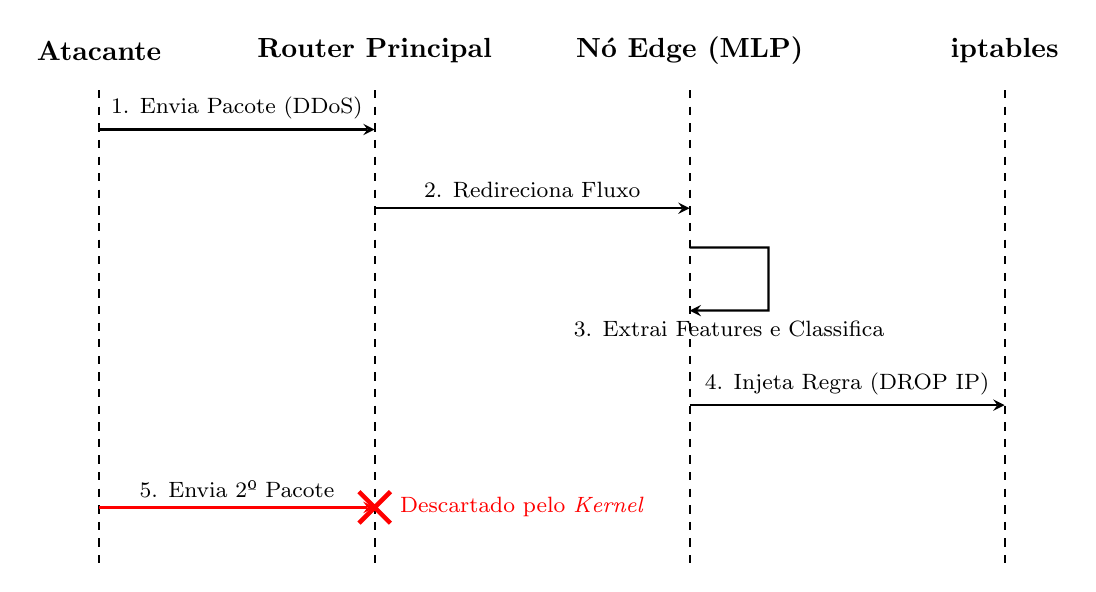
\begin{tikzpicture}[>=stealth]
        % Atores (Lifelines)
        \node (h1) at (0,0) {\textbf{Atacante}};
        \node (router) at (3.5,0) {\textbf{Router Principal}};
        \node (edge) at (7.5,0) {\textbf{Nó Edge (MLP)}};
        \node (firewall) at (11.5,0) {\textbf{iptables}};

        % Linhas Verticais de Tempo
        \draw[thick, dashed] (0,-0.5) -- (0,-6.5);
        \draw[thick, dashed] (3.5,-0.5) -- (3.5,-6.5);
        \draw[thick, dashed] (7.5,-0.5) -- (7.5,-6.5);
        \draw[thick, dashed] (11.5,-0.5) -- (11.5,-6.5);

        % Comunicações (Mensagens)
        \draw[->, thick] (0,-1) -- node[above, font=\footnotesize] {1. Envia Pacote (DDoS)} (3.5,-1);
        \draw[->, thick] (3.5,-2) -- node[above, font=\footnotesize] {2. Redireciona Fluxo} (7.5,-2);

        % Processamento interno no Edge
        \draw[->, thick] (7.5,-2.5) -- ++(1,0) -- ++(0,-0.8) -- node[below, font=\footnotesize] {3. Extrai Features e Classifica} (7.5,-3.3);

        % Aplicação de mitigação
        \draw[->, thick] (7.5,-4.5) -- node[above, font=\footnotesize] {4. Injeta Regra (DROP IP)} (11.5,-4.5);

        % Segunda tentativa do atacante (Bloqueado)
        \draw[->, thick, red] (0,-5.8) -- node[above, text=black, font=\footnotesize] {5. Envia 2º Pacote} (3.5,-5.8);

        % Cruz de bloqueio no Router
        \draw[xshift=3.5cm, yshift=-5.8cm, ultra thick, red] (-0.2,-0.2) -- (0.2,0.2) (-0.2,0.2) -- (0.2,-0.2);
        \node[right, text=red, font=\footnotesize] at (3.7, -5.8) {Descartado pelo \textit{Kernel}};

    \end{tikzpicture}
    \caption{Diagrama de Sequência ilustrando a interceção e o bloqueio de um ataque na periferia da rede.}
    \label{fig:diagrama_sequencia}
\end{figure}
